%% moderncv-cover-letter.tex (compiled with pdfLaTeX)
%% Copyright 2024 Christine P. Chai
%
% This work may be distributed and/or modified under the
% conditions of the LaTeX Project Public License version 1.3c,
% available at https://spdx.org/licenses/LPPL-1.3c.html.

% Customized ModernCV template developed by Christine P. Chai
% Built upon the moderncv package from Xavier Danaux

\documentclass[10pt,letterpaper,sans]{moderncv}        % possible options include font size ('10pt', '11pt' and '12pt'), paper size ('a4paper', 'letterpaper', 'a5paper', 'legalpaper', 'executivepaper' and 'landscape') and font family ('sans' and 'roman')
%\usepackage[spanish,es-lcroman]{babel}

%----------------------------------------------------------------------------------------
%	PACKAGES AND OTHER DOCUMENT CONFIGURATIONS
%----------------------------------------------------------------------------------------

% moderncv themes
\moderncvstyle{classic}                            % style options are 'casual' (default), 'classic', 'oldstyle' and 'banking'
\moderncvcolor{blue}                              % color options 'blue' (default), 'orange', 'green', 'red', 'purple', 'grey' and 'black'
%\renewcommand{\familydefault}{\sfdefault}         % to set the default font; use '\sfdefault' for the default sans serif font, '\rmdefault' for the default roman one, or any tex font name
%\nopagenumbers{}                                  % uncomment to suppress automatic page numbering for CVs longer than one page

% character encoding
\usepackage[utf8]{inputenc}                       % if you are not using xelatex ou lualatex, replace by the encoding you are using
%\usepackage{CJKutf8}                              % if you need to use CJK to typeset your resume in Chinese, Japanese or Korean

% adjust the page margins
\usepackage[scale=0.90]{geometry}
%\setlength{\hintscolumnwidth}{3cm}                % if you want to change the width of the column with the dates
%\setlength{\makecvtitlenamewidth}{10cm}           % for the 'classic' style, if you want to force the width allocated to your name and avoid line breaks. be careful though, the length is normally calculated to avoid any overlap with your personal info; use this at your own typographical risks...

% horizontal alignment
\usepackage{etoolbox}% http://ctan.org/pkg/etoolbox
\makeatletter
\patchcmd{\makelettertitle}% <cmd>
  {\raggedright \@opening}% <search>
  {\@opening}% <replace>
  {}{}% <success><failure>
\makeatother

% personal data
\name{Firstname}{Lastname}
%\title{Resumé title}                               % optional, remove / comment the line if not wanted

% All information in this block is optional, comment out any lines you don't need
%\title{Firstname CV}
\address{P.O. Box xxxxx, City, State, Zip Code}{}
%\address{P.O. Box 25142, Arlington, VA 22202}{}
\mobile{(111) 111-1111}
\email{firstname.lastname@gmail.com}
\homepage{(put your url here)}

\extrainfo{%
\httplink{www.linkedin.com/in/yourname}\\
\httplink{github.com/yourGitHubID}
}

%\photo[64pt][0.4pt]{picture}                       % optional, remove / comment the line if not wanted; '64pt' is the height the picture must be resized to, 0.4pt is the thickness of the frame around it (put it to 0pt for no frame) and 'picture' is the name of the picture file
%\quote{Some quote}                                 % optional, remove / comment the line if not wanted

% to show numerical labels in the bibliography (default is to show no labels); only useful if you make citations in your resume
%\makeatletter
%\renewcommand*{\bibliographyitemlabel}{\@biblabel{\arabic{enumiv}}}
%\makeatother
%\renewcommand*{\bibliographyitemlabel}{[\arabic{enumiv}]}% CONSIDER REPLACING THE ABOVE BY THIS

% bibliography with mutiple entries
%\usepackage{multibib}
%\newcites{book,misc}{{Books},{Others}}
%----------------------------------------------------------------------------------
%            content
%----------------------------------------------------------------------------------
\begin{document}
%-----       letter       ---------------------------------------------------------
% recipient data
\recipient{Company Name}{Data Science Division}
\date{\today}
\opening{Dear Hiring Manager,}
\closing{Best regards,\\
  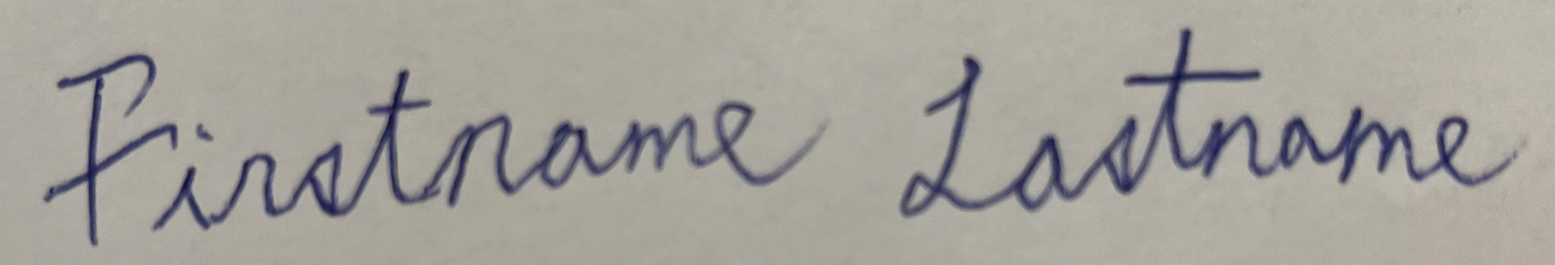
\includegraphics[width=4cm]{signature.png}  \vspace{-1cm}}

%\enclosure[Adjunto]{CV}          % use an optional argument to use a string other than "Enclosure", or redefine \enclname
\makelettertitle

Lorem ipsum dolor sit amet, consectetur adipiscing elit. Nunc tortor dui, blandit et laoreet bibendum, tempor rhoncus lectus. Nullam id egestas quam. Donec non egestas tortor, vitae malesuada nulla. Nam semper mattis justo. Nullam lobortis tincidunt urna, vitae cursus est tincidunt quis. Duis dignissim ex ut enim lobortis, vitae consectetur nulla pharetra. Suspendisse pulvinar leo massa, eget porttitor justo pharetra sit amet. Donec vitae lorem non risus finibus viverra id non nulla. Donec rhoncus nisi id diam feugiat porttitor. Nunc volutpat risus vitae dignissim molestie.

\vspace{10pt}

Donec id dignissim nibh. Nunc bibendum leo sed congue lobortis. Donec eget magna commodo, consectetur risus quis, elementum orci. Proin iaculis dapibus massa eget vestibulum. Vestibulum felis magna, volutpat a enim at, venenatis condimentum nulla. Praesent eros sapien, rhoncus at viverra non, posuere a libero. Maecenas mattis, ligula eget ultrices varius, orci mauris ultricies neque, quis cursus arcu tellus eu elit. Proin ligula nunc, finibus eu porta at, auctor vel mauris. Phasellus fermentum velit sit amet posuere lacinia. Duis ipsum tortor, viverra vel nisi in, pulvinar tristique quam. Nam et iaculis turpis, nec blandit urna. Ut condimentum ultrices nisi. Phasellus ac malesuada erat. Phasellus et ultrices est. Phasellus vitae diam faucibus, luctus dui sed, consectetur justo. Sed eu erat at nisl faucibus lacinia quis quis massa. Donec nulla tellus, mollis vitae risus a, vulputate dapibus sapien. Duis pretium at purus eu lobortis. Morbi accumsan consectetur leo, in molestie quam elementum id. Fusce ac purus at elit facilisis mattis ut nec ante. Vivamus consectetur, nulla quis iaculis dictum, nulla tellus tristique orci, non lacinia metus elit a metus. Proin sed purus vestibulum, sodales orci id, volutpat tortor. In viverra pulvinar sagittis.

\vspace{10pt}

Nullam vulputate sollicitudin justo quis gravida. Fusce eleifend diam ut facilisis interdum. Etiam pharetra dignissim nisl, a varius risus cursus vel. Proin fringilla leo augue, nec finibus turpis hendrerit eu. Integer faucibus dolor ut odio consectetur, ac interdum ligula mollis. Interdum et malesuada fames ac ante ipsum primis in faucibus. Aenean faucibus nibh facilisis mauris cursus, vel lobortis ligula faucibus. In eu diam id lectus condimentum viverra. In eget tincidunt purus, sed rutrum dolor. Phasellus molestie neque metus, et placerat ex sollicitudin eu. Suspendisse non ullamcorper erat. Vestibulum eu eleifend ex. Aenean ullamcorper massa eget maximus aliquet. Curabitur placerat quis lacus nec maximus. Nullam leo diam, tincidunt id ante nec, ultricies finibus odio. Morbi a fermentum mauris. Fusce vel mi mi. Sed vitae nisi mollis, ultricies enim ut, pellentesque nisi. Nam suscipit aliquam turpis, euismod tristique est vestibulum et. Morbi fermentum urna sed quam tincidunt ornare. Vestibulum tellus tortor, vehicula nec euismod et, venenatis quis sem. Sed quis orci urna. Nunc efficitur lorem et facilisis tristique. Mauris lacinia odio consectetur turpis congue fringilla.

\vspace{10pt}

Cras ac dui posuere, interdum lectus quis, aliquam enim. Cras at laoreet nunc. Sed sed egestas arcu. Morbi elementum sodales est sit amet pellentesque. Cras nec mi sem. Etiam at faucibus augue. Vestibulum eu massa ullamcorper, sodales lacus sit amet, consectetur risus. Curabitur id pulvinar orci, vel feugiat ipsum. Nullam interdum turpis et sem cursus, a ullamcorper est vestibulum. Vivamus bibendum orci nulla, in ultrices ante accumsan at. Phasellus interdum volutpat metus, at lacinia quam dictum a. Nam a risus tempus, ultricies risus id, facilisis nunc. Donec a consectetur odio. Aliquam placerat molestie ante, at varius lorem dignissim in. Aenean maximus bibendum erat at pellentesque. In et ipsum vel justo pretium ultrices. Duis porttitor rhoncus nulla id aliquam.

\vspace{10pt}

Vestibulum vitae justo ac tellus tempor commodo sit amet vel nisi. Sed lacinia consectetur nisl, pellentesque cursus dolor semper eget. Cras id congue libero. Pellentesque habitant morbi tristique senectus et netus et malesuada fames ac turpis egestas. Etiam at posuere eros. Nulla ut felis enim. Integer vitae vehicula tortor. Mauris enim tellus, fringilla vitae varius et, vestibulum aliquet purus. Phasellus sit amet ligula vitae eros imperdiet gravida. Vivamus risus eros, feugiat non semper eget, sagittis pretium libero. Vestibulum euismod sit amet urna vitae euismod. Etiam tincidunt hendrerit mi in mollis. Suspendisse a accumsan sem. Aliquam tempor euismod felis, eu maximus lorem tristique eu. Sed ut semper nibh.

\vspace{10pt}

\makeletterclosing

\end{document}

%% end of file `template.tex'.